3.1  コイル\\
  本実験の\(g\)因子測定において、磁場をコイルから発生させた。コイルは2004年度P1の課題研究用に作成されたものを使用した。このコイルはMainコイルとして4つのコイルを並列でつないだものを並べ、さらに2つのSubコイルを用いたものを使用した。
Mainコイルには31.0Vで19.0A、sub1コイルには3.5Vで0.80A、sub2コイルには3.6Vで0.80Aの電流を流した。
\begin{figure}[htbp]
 \begin{center}
  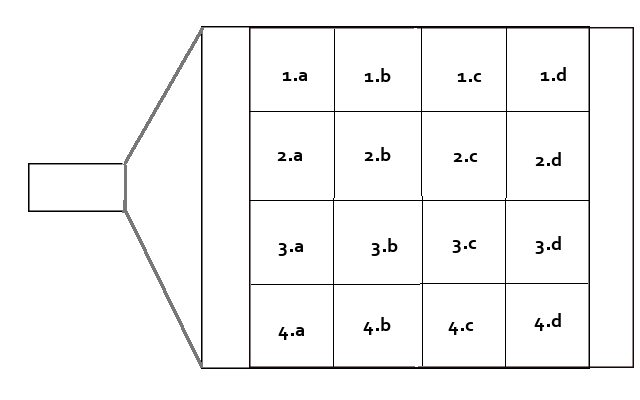
\includegraphics[width=100mm]{coil.xcf}
  \caption[width=100mm]{coil.tex}
 \end{center}
\end{figure}
磁場の測定では、コイルに電流を流してから24時間経過して磁場が安定したあと、
測定位置を銅板が入っている部分を銅板の大きさが縦50cm横48cmなので、上図のように16のセクションに分け、それぞれの場所においての磁場を計3回測定した。
その測定結果を下表に記す。
\begin{center}
\begin{tabular}{c|ccc|c}\hline
  セクション&1回目[Gauss]&2回目[Gauss]&3回目[Gauss]&3回の平均[Gauss]\\ \hline
  1.a & 51.0 & 47.0 & & \\
  1.b & 53.0 & 50.1 & & \\
  1.c & 51.6 & 50.4 & & \\
  1.d & 49.6 & 49.7 & & \\
  2.a & 54.7 & 49.2 & & \\
  2.b & 55.2 & 49.5 & & \\
  2.c & 53.2 & 49.0 & & \\
  2.d & 50.2 & 49.8 & & \\
  3.a & 51.2 & 48.8 & & \\
  3.b & 50.2 & 48.9 & & \\
  3.c & 49.8 & 48.3 & & \\
  3.d & 49.6 & 47.7 & & \\
  4.a & 50.6 & 48.0 & & \\
  4.b & 49.2 & 49.4 & & \\
  4.c & 51.5 & 47.4 & & \\
  4.d & 49.8 & 48.4 & & \\
\end{tabular}
\end{center}
